\documentclass[main.tex]{subfiles}
\begin{document}

\section*{Introduction and relevant material}

These are the
(yet to be)
revised notes for the course ``Fundamentals of Astrophysics and Cosmology'' held by professor Sabino Matarrese in fall 2019 at the university of Padua.

They are based on the notes I took during lectures, complemented with notes from the previous years.

They will be revised by the professor in the future, as of yet they have not.

The exam is a traditional oral exam, there are fixed dates but they do not matter: on an individual basis we should write an email to the professor to set a date and time.

\paragraph{Material}

There is a dropbox folder with notes by a student from the previous years \cite[]{Pacciani:2018} and handwritten notes by the professor.

There are many good textbooks, for example ``\citetitle{LucchinColes:2002}'' by \citeauthor{LucchinColes:2002} \cite[]{LucchinColes:2002}.

% Sabino Matarrese \(\heartsuit\).

% On the astroparticle side, there is another book: I did not catch its name.


% In october the lessons of GR and this course on fridays are swapped.

\chapter{Cosmography}

% \section*{3 October 2019}
\marginpar{Thursday\\ 2019-10-3, \\ compiled \\ \today}

\section{The cosmological principle}

The basis for the modern treatment of cosmology is the \textbf{cosmological principle} (or Copernican principle):
roughly stated, it is ``\emph{we do not occupy a special, atypical position in the universe}''.
We will discuss the validity of this later in this section.
It is extremely useful to make such an assumption since it endows our model of the universe with a great deal of symmetry, which makes its mathematical treatment manageable. 

A more formal statement is:
%
\begin{proposition}[Cosmological principle]
    Every \emph{comoving observer} observes the Universe around them at a \emph{fixed time} in their reference frame as being \emph{homogeneous} and \emph{isotropic}.
\end{proposition}

\textbf{Comoving} means moving coherently with the absolute reference frame, which is defined as the rest frame of the cosmic fluid, which determines the geometry of the universe. 

When we observe the Cosmic Microwave Background (CMB) we see that we are surrounded by radiation distributed like a blackbody of temperature \(T _{\text{CMB}} \approx \SI{2.725}{K}\) \cite[]{Fixsen:2009}.

This radiation is not uniformly distributed in the sky: we 
see a \emph{dipole modulation} of around \(\Delta T \approx\)\SI{3.4}{mK} \cite[]{PlanckCollaboration:2018I}.
This is due to the Doppler effect: the Solar System is \emph{not} comoving with respect to the CMB.

In fact, we can measure the \emph{peculiar velocity} of the Solar System this way: it comes out to be around \(c \Delta T / T _{\text{CMB}} \approx \SI{370}{km/s}\).
This cannot be explained by the movement of the Sun through the galaxy, nor by the movement of the galaxy through the Local Group: the Local group is actually moving with respect to the absolute reference.
In fact, the velocities of the Sun with respect to the Local Group and the velocity of the Local Group with respect to the CMB are almost directed in opposite directions, so the velocity of the LG with respect to the CMB can be measured to be \(\approx \SI{620}{km/s}\) \cite[Table 3]{PlanckCollaboration:2018I}.

So, the absolute reference frame can be experimentally defined as the frame of the observer who sees the CMB with zero dipole moment.

The CMB has anisotropies of the order of \SI{20}{\micro K} (root mean square) \cite[]{Wright:2003} at higher order multipole moments: it is uniform to approximately 1 part in \num{e5}.

% The velocity needed to explain the Doppler effect is of the order of \SI{630}{\kilo\metre\per\second}.
% This is \emph{after} correcting for the motion of everything up to a galactic scale.

% So, we must assume that to get a \emph{comoving} observer we should launch it in a certain direction at an extremely high velocity. So, we \emph{do} have a preferred frame.

The word ``time'' in \textbf{fixed time} refers to the proper time of a comoving observer, which is called \emph{cosmic time}.

% This refers to scales on the order of \SI{100}{\mega\parsec}.

\textbf{Homogeneity} means that the characteristics of the universe as observed from a point are the same as they would be as observed from any other point. 

\textbf{Isotropy} means that the characteristics of the universe as observed in a certain direction are the same as they would be if they were observed in another direction.

\paragraph{On the validity of the cosmological principle}

The principle is expected to hold only on very large\footnote{Larger than \(260 h^{-1} \SI{}{Mpc} \approx \SI{380}{Mpc}\) \cite[]{Yadav+:2010}, where \(h \approx \num{.68}\) \cite[]{PlanckCollaboration:2016XIII}: this will be made clearer in later sections, but is meant to give an idea of the length scales involved.} scales:
at small scales we see structures, such as galaxies or our Solar System, so we surely do not have homogeneity.

How can we talk about homogeneity if we can only look at the universe from a single point?
We must \emph{assume} that any other observer would also see isotropy as we do.

Isotropy around every point implies homogeneity. We observe isotropy, we assume homogeneity.
So, we can go from isotropy to homogeneity under the assumption that we are typical observers.

% What if we are not typical? a different assumption is that our observer status is \emph{random} according to some distribution\dots
% This discussion then starts to involve the anthropic principle.

In the end, this assumption has to be made before any cosmological study starts: it might not be completely correct, but it allows us to make falsifiable predictions, so we shall keep it until the models it allows us to create do not match observations anymore.

\section{The geometry of spacetime}

The best description for gravity we have so far is given by the general theory of relativity (GR).
In it, spacetime is modelled as a 3+1-dimensional semi-Riemannian manifold with a line element which is  generally given by the expression \(\dd{s^2} = g_{ab} \dd{x^a} \dd{x^b} \) and which.

Latin indices can take values from 0 to 3, and we adopt the ``mostly minus'' metric signature.

Such a spacetime can have up to \(4(4+1) / 2 = 10\) global continuous symmetries, which can be classified into:
\begin{enumerate}[label=(\alph*)]
  \item 1 time translation; \label{item:time-translation}
  \item 3 Lorentz boosts; \label{item:lorentz-boost}
  \item 3 spatial translations; \label{item:spatial-translation}
  \item 3 spatial rotations. \label{item:spatial-rotation}
\end{enumerate}

The metric of Minkowski spacetime, which has all of these 10 symmetries, reads: 
%
\begin{subequations}
\begin{align}
\dd{s^2} &= c^2 \dd{t^2} - \dd{\vec{x}^2} && \text{(cartesian coordinates)} \\
&= c^2 \dd{t^2} - \dd{r^2} - r^2 \dd{\Omega^2} && \text{(spherical coordinates)}
\,,
\end{align}
\end{subequations}
%
where \(r = \abs{x}\), while \(\theta \) and \(\varphi \) are the spherical angles and \(\dd{\Omega^2} = \dd{\theta^2} + \sin^2\theta \dd{\varphi^2 }\).

In cosmology we lose time translation symmetry, since the universe is expanding, and Lorentz boost symmetry, since as we saw in the previous section we can tell at which speed we are moving with respect to the CMB.

We keep the purely spatial symmetries: so, our description of spacetime will be as a 3+1-dimensional manifold which, if we fix the temporal coordinate for a comoving observer, reduces to a \emph{maximally symmetric} 3-dimensional space --- for 3 dimensions the maximum number of symmetries is \(3(3+1) / 2 = 6\), which correspond to \ref{item:spatial-translation} and \ref{item:spatial-rotation}. 

It can be shown that the most general form of a metric satisfying these conditions is the \textbf{Friedmann-Lemaître-Robertson-Walker line element},\footnote{This is sometimes called just ``Robertson-Walker'', or RW, or FLRW.} which, in the comoving frame, reads
%
\boxalign{
\begin{align} \label{eq:robertson-walker}
  \dd{s^2} = c^2 \dd{t^2} - a^2(t) \qty(\frac{\dd{r^2}}{1 - k r^2} + r^2 \dd{\Omega^2} )\,.
\end{align}}
%
% Sometimes it is convenient to write \(\dd{\theta^2} + \sin^2(\theta) \dd{\varphi^2} = \dd{\Omega^2}\).

% The angular part is the same (just rescaled) as the Minkowski one.

The coordinate \(r\) does not have the dimensions of a length: we choose our variables so that \(a(t)\) is a length, while \(r\) is adimensional.\footnote{This is a matter of convention: if we normalize \(\abs{k}=1\) then we will have \(0 \leq r < 1\); we could also let \(k\) be arbitrarily large; then \(r\) would also be.}

The parameter \(a(t)\) is called the \emph{scale factor}: varying it amounts to rescaling all of space.
It has the dimensions of a length, and it depends on the cosmic time \(t\).

The parameter \(k\) is a constant describing the spatial curvature, which can always be normalized to \(\pm 1\) or \(0\).
Universes with:
\begin{itemize}
    \item \(k=1\) are called closed universes;
    \item \(k=-1\) are called open universes;
    \item \(k=0\) are called flat universes.
\end{itemize}

We can choose the normalization of \(k\), but its sign is a constant.
Positive values correspond to \(k=1\), negative values to \(k=-1\).
When computing probability distributions for \(k\), we must not consider it to be a discrete variable but a continuous variable instead: so, the set of flat universes with \(k=0\) has zero measure, and thus zero probability with any probability density function.

% In a 4D flat spacetime we have the 10 degrees of freedom of Lorentz transformations: Minkowski spacetime is \emph{maximally symmetric}.

% Other possible geometries are De Sitter and Anti de Sitter spacetimes.

% For the actual universe, however, not all of these symmetries hold: the universe seems not to be symmetric under time translation, and we have a preferential velocity.
% 4 symmetries are broken (time translation and Lorentz boosts), 6 hold (rotations and spatial translations): our assumption is that there is a 3D maximally symmetric space.

% Under these assumptions, we can derive the RW line element.

\subsection{A bidimensional example}

We consider surfaces: these are the simplest manifolds which can have intrinsic curvature.

\begin{bluebox}
Intrinsic curvature is described by the Riemann tensor, which has 20 independent components in 4D and 6 in 3D, so it is difficult to visualize.

On the other hand, in 2D has only 1 independent component: \(R_{1212} = R \det g_{ab}\), where \(R\) is the scalar curvature. 

\(R\) has an immediate geometric interpretation: it is equal to \(2/(R_1 R_2)\), where \(R_i\) are the radii of the osculating circles at the point; it is positive if the circles are in the same direction, as they are for a sphere, and negative if they are in different directions, as they are for a hyperboloid.

If we have a direction in which the surface is flat, such as in a cylinder, then \(R=0\): it is intrinsically flat.
\end{bluebox}

The metric for a cartesian flat 2D plane is \(\dd{l^2} = a^2 (\dd{r^2} + r^2 \dd{\theta^2}) \).
The constant \(a\) is included since we want \(r\) to be adimensional.

The metric for the surface of a sphere is:
\(\dd[]{l^2} = a^2 \qty(\dd[]{\theta^2} + \sin^2 \theta \dd[]{\varphi^2}) \),
where \(a^2 = R^2\), the square radius of the sphere.

The metric for the surface of a hyperboloid is:
\(\dd[]{l^2} = a^2 \qty(\dd[]{\theta^2} + \sinh^2 \theta \dd[]{\varphi^2}) \),
therefore the only difference is that trigonometric functions become hyperbolic ones.

\begin{figure}[ht]
\centering
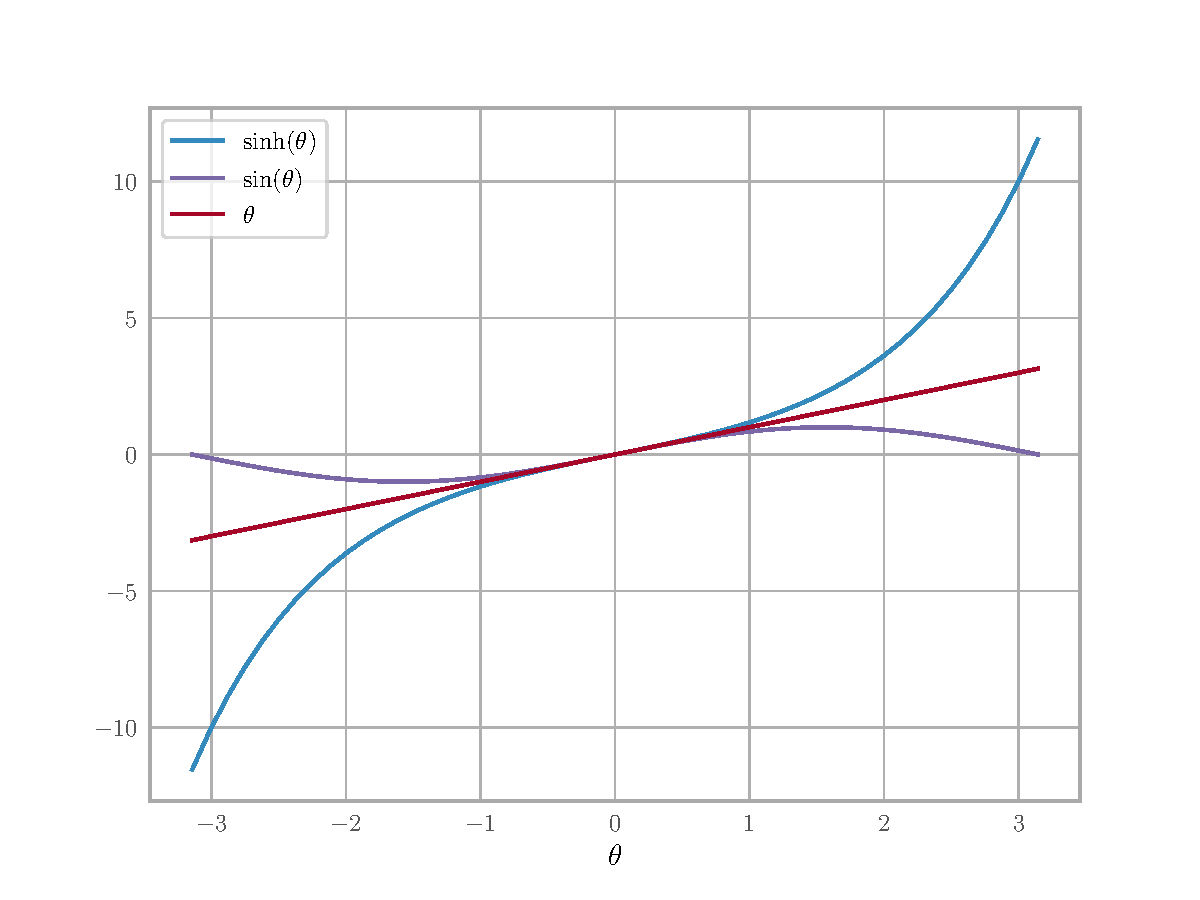
\includegraphics[width=\textwidth]{figures/sin_vs_sinh.pdf}
\caption{Plot of the functions \(\sin(\theta )\) and \(\sinh (\theta )\) in the interval \(-\pi \leq \theta\leq \pi  \).}
\label{fig:sin_vs_sinh}
\end{figure}

Do note that for the sphere \(\theta  \in [- \pi, \pi ]\) while for the hyperboloid we can in principle have \(\theta \in \mathbb{R}\): this is indicative of the fact that the sphere is bounded, while the hyperboloid is infinite, 

For both of these, let us define the variable: \(r = \sin\theta \) in the spherical case, and \(r = \sinh \theta \)  in the hyperbolic case.

As we change variable we do the following manipulation for the sphere: 
%
\begin{subequations}
\begin{align}
\dd{r^2} &= \qty(\dv{r}{\theta })^2 \dd{\theta^2} = \cos^2\theta \dd{\theta^2}  \\
\implies \dd{\theta^2} &= \frac{\dd{r^2}}{\cos^2\theta } = \frac{\dd{r^2}}{1 - r^2}
\,,
\end{align}
\end{subequations}
%
and similarly for the hyperboloid, except for the fact that in that case \(\cosh^2 \theta  = 1 + \sinh^2\theta = 1+r^2 \).

So, the line elements become respectively:
\begin{subequations}
\begin{align}
    \dd[]{l^2}_{\text{sphere}} &= a^2 \qty(\frac{\dd[]{r^2}}{1 - r^2}  + r^2 \dd{\varphi^2}  )\\
    \dd[]{l^2}_{\text{hyperboloid}} &= a^2 \qty(\frac{\dd[]{r^2}}{1 + r^2} + r^2 \dd{\varphi^2}  )\,.
\end{align}
\end{subequations}

We have a striking similarity to the Robertson-Walker metric: we only need to make the substitution \(\dd{\varphi } \rightarrow \dd{\Omega }\) in order to recover it.

We can also work backwards and rewrite the RW line element in sphere- or hyperboloid-like coordinates:
\begin{equation}
  \dd{l^2} = c^2 \dd{t^2} - a^2 \begin{cases}
      \dd{\chi^2} + \sin^2 \chi \dd{\Omega^2} \\
      \dd{\chi^2} + \chi^2\dd{\Omega^2} \\
      \dd{\chi^2} + \sinh^2 \chi \dd{\Omega^2}
\end{cases}
\end{equation}
%
where we introduce a variable \(\chi \) defined so that if \(k = +1\) then \(r = \sin \chi\), if \(k=0\)  then \(r=\chi\), and if \(k = -1\) then \(r = \sinh \chi\).

The properties of the sphere and of the hyperboloid actually carry over to the 3D case: a spacetime with positive curvature is bounded, while if it is flat or hyperbolic it is unbounded.

\subsection{Other forms of the RW metric}

If we wish to use cartesian coordinates the RW metric takes the following expression:
%
\begin{equation}
  \dd{s^2} = c^2 \dd{t^2} - a^2 (t) \qty(1 + \frac{k \abs{x}^2}{4} )^{-2} \qty(\dd{x^2} + \dd{y^2} + \dd{z^2}) \,.
\end{equation}

Universes in which \(a\) is a constant are called \emph{Einstein spaces}.

We can also change time variable: the \emph{conformal time} \(\eta \) is such that \(\dd{t} = a(\eta) \dd{\eta} \), where \(a(\eta) \defeq a(t(\eta))\): so, we will have

\begin{equation}
  \dd{s^2} = a^2 (\eta) \qty(c^2 \dd{\eta^2} - \qty(\frac{\dd{r^2}}{1 - kr^2} + r^2 \dd{\Omega})) \,.
\end{equation}

% The parameter \(\eta\) is called \emph{conformal time}: RW is said to be \emph{conformal} to Minkowski.
\begin{bluebox}
Conformal transformations are defined to be those which preserve angles locally; since angles are defined through the metric but the angle between two vectors does not change if they are rescaled, this can be translated into the condition that the metric is rescaled by a generic function:
%
\begin{align}
g_{ab} \rightarrow a^2(x^{i}) g_{ab}
\,.
\end{align}

In our case, the dependence on the point in spacetime is reduced to a dependence on the cosmic time only since we have symmetry with respect to spatial translations.
\end{bluebox}

In general our spacetime does not have conformal symmetry: a generic massive particle in it has a Compton wavelength \(\lambda = h / (mc)\) which defines its interaction cross section, so if the spacetime expands an ensemble of these particles will have different dynamics.

However, conformal geometry is useful for the description of particles which have no characteristic length, such as photons.
The photons of the CMB look like they are thermal: they were thermal in the early universe, since they were in thermal equilibrium with matter (photons and matter particles were constantly Compton-scattering off each other); when matter and radiation decoupled the photons scattered for the last time and then kept travelling.
The universe has since expanded by a factor \(\approx 1090\), but because of the fact that the photons do not have a characteristic length their distribution can still be modelled as a blackbody distribution for an appropriately rescaled temperature.

\section{The energy budget of the universe}

Up until now we did not consider any dynamics in our spacetime. We will discuss this topic in more detail in later sections, but for now we give the result: the dynamics of the universe are described by the Friedmann equations:
%
\begin{subequations} \label{eq:friedmann-equations} 
\begin{align}
    \dot{a}^2 &= \frac{8 \pi G_N }{3} \rho a^2 - kc^2  \label{eq:friedmann-1}\\
    \ddot{a} &= - \frac{4 \pi G_N }{3} a  \qty(\rho  + \frac{3P}{c^2} )  \label{eq:friedmann-2}\\
    \dot{\rho} &= -3 \frac{\dot{a} }{a} \qty(\rho + \frac{P}{c^2} ) \label{eq:friedmann-3}
\end{align}
\end{subequations}
%
where dots denote differentiation with respect to the \emph{cosmic time} \(t\), \(G_N\) is Newton's gravitational constant, \(\rho = \rho( t) \) is the energy density, and \(P = P(t)\) is  the isotropic pressure.

The curvature \(k\) appears in the first equation: so we can try to measure it by comparing the other two terms in the equations.
This way, we can determine whether the universe is flat or curved.

In order to discuss this problem, let us establish some notation: an important parameter is \(H(t) \defeq \dot{a} / a\), the \emph{Hubble parameter}.
We can write an equation for it from the first Friedmann one:
%
\begin{equation} \label{eq:hubble-parameter-evolution}
  H^2 = \frac{8 \pi G}{3} \rho - \frac{kc^2}{a^2}
\end{equation}

If \(k=0\), then there we must have a critical energy density 
%
\begin{align}
  \rho_C (t) = 3 H^2 (t) / (8 \pi G)
\,,
\end{align}
%
and we define \(\Omega(t) = \rho(t) / \rho_C(t)\).
For a flat universe, \(\Omega = 1\), and so we can determine \(k = \sign (\Omega -1)\), since: 
%
\begin{align}
1 &= \frac{8 \pi G}{3} \frac{\rho }{H^2} - k \frac{c^2}{a^2H^2}  \marginnote{Dividing 
equation \eqref{eq:hubble-parameter-evolution} 
through by \(H^2\)}\\
\frac{\rho }{\rho_{c}} - 1 &= k \frac{c^2}{a^2H^2}  \\
\sign (\Omega -1) &= \sign \qty(k \frac{c^2}{a^2H^2}) = \sign (k) = k \marginnote{Took sign of both sides}
\,.
\end{align}

The alternative is measuring \(k\) directly, say, by drawing really large triangles and measuring the sum of their internal angles.
The latter is a ``Newtonian'' measurement, while the former is a ``GR'' measurement. The Newtonian measurement is much harder to perform.

% This computation also proves that the spatial curvature is constant throughout the history of the universe: 

Further, we define the \textbf{Hubble parameter}:
\begin{equation}
  H_0 = H(t_0) = 100 h \times \SI{}{\kilo\metre\per\second\per\mega\parsec}
  \approx \SI{70}{\kilo\metre\per\second\per\mega\parsec}
\end{equation}
%
where \(h \approx \num{.7}\) is a number, and \(t_0\) just means \emph{now}.\footnote{Also, \SI{}{pc} means ``parsec'': 
%
\begin{align}
\SI{1}{pc} = \frac{\SI{1}{AU}}{\SI{1}{arcsec}}
\approx \SI{3.085e+16}{m}
\approx \SI{3.26}{ly}
\,,
\end{align}
%
where the angle is to be interpreted as adimensional (in radians), and \SI{}{AU} is an astronomical unit, the Earth-Sun average distance. 
The definition is as such because of a way we have to measure the distances to nearby objects, by measuring their parallax between winter and summer: if they are close enough, they will have apparently moved with respect to further objects, because of the movement of the Earth around the Sun.}

The reason for this peculiar way to write the constant is that historically it has been difficult to determine the value of \(H_0 \) precisely, and it affects many astronomical conversions: keeping it indeterminate in this way allows us to quickly update our old estimates if we measure \(H_0 \) more precisely later.
Historically, in the American school, the pupils of Hubble thought \(h \sim 0.5\), while the French school thought \(h \sim 1\).
Now, a great issue in cosmology is the disagreement between the measurements of \(H_0 \) obtained from the cosmic distance ladder and those obtained from the CMB \cite[]{Wong:2019}.

\subsection{Energy density}

So, in order to determine the spatial curvature of the universe we need to look at \(\Omega \propto \rho \): so, we need to measure the energy density of the universe.

How do we do it?

Let us start by considering the energy density \emph{today} (index 0) due to \emph{galaxies} (index \(g\)): \(\rho_{0g}\).
We do not directly observe the mass\footnote{Here the terms mass and energy are used equivalently: the velocity of galaxies with respect to the CMB is nonrelativistic, so we approximate \(E = \gamma m c^2 \approx m c^2\).}  
of galaxies: we can only measure their luminosities.

So, we do the following: we compute the mean value of \(\rho \), the mass per unit volume, with the aid of the galaxy luminosity per unit volume \(\ell\): we find 
%
\begin{align}
\expval{\rho }
&= \expval{\ell \,\frac{\rho }{\ell}} 
= \expval{\ell} \expval{\frac{\rho }{\ell}} 
= \expval{\ell} \expval{\frac{M}{L}}
\,,
\end{align}
%
where \(\expval{M  / L}\) is the average ratio of mass over luminosity per galaxy: we had a ratio of densities, but since we are considering averages we can integrate above and below with respect to the spatial volume.

\todo[inline]{In order to simplify the expression, we assume that the \(\rho / \ell\) ratio is uncorrelated to the luminosity per unit volume \(\ell\): is there a justification for this, beyond saying that it is true by homogeneity?}

It is measured in units of solar mass over solar luminosity: \(M_{\odot} / L_{\odot}\).
Reference values for these are \(M_{\odot} \sim \SI{1.99e33}{g}\), while \(L_\odot \sim \SI{3.9e33}{\erg\per\second} \).

We denote \( \expval{\ell} \defeq \mathscr L_g  \): it is the mean (intrinsic, bolometric\footnote{Bolometric means ``total, over all wavelengths'', as opposed to the luminosity in a certain wavelength band, which is easier to measure in astronomy.}) luminosity of galaxies per unit volume.

By definition, it is given by 
%
\begin{equation}
  \mathscr L _g = \int_0^\infty  L \Phi(L) \dd{L}
\,,
\end{equation}
%
where \(\Phi(L)\) is the number density of galaxies per unit volume and unit luminosity: the \emph{luminosity function}.
% With of our observations we estimate the shape of \(\Phi(L)\).
% We know that the integral must converge, so we can bound the shape of \(\Phi\).

\end{document}
